\chapter{Background}
\label{cha:background}

In this section, there will be all the background information relevat to the thesis,
that are required in order to properly understand the matter of the project, the
problem, the technologies and the solution.

We will start in subsection \ref{cha:CPU speculation contract} by explaining
what a CPU speculation contract is, and why it is important for the scope of this
thesis. Then we will then move to subsection \ref{cha:Revizor}, where we will talk
about the Revizor tool, that is used in the research project to detect the
contract of a CPU. We will detail how it works and some background information.
In subsection \ref{cha:Rosette}, we will talk about Rosette, the solver-aided
programming language that is used to encode the violations reported from Revizor.
With this tool we are able to feed the loop, that is the base of this project. In
subsection \ref{cha: Loop outlook}, we will give an overview of the loop that is
used to synthesize the CPU contract, using all the tools and language discussed in
previous sections, and therefore deeper explaing the research project this
thesis is part of. In subsection \ref{cha:DSL}, we will talk about the Domain
Specific Language (DSL) that the team used before this thesis's project, and why
it was not enough for the scope of the overall project. In subsection
\ref{cha:BIR}, we will talk about the Binary Intermediate Representation (BIR) language,
that has been chosen to replace the DSL. Also, in \ref{cha:Language comparison}
there will be a more in-depth comparison and explaination of the differences
between the two languages, with a brief about why BIR demostred to be the best choice
for this project and this whole domain.

\section{CPU speculation contract}
\label{cha:CPU speculation contract} Before diving into what a CPU speculation contract
is, it is better to have a clear idea of what speculative execution is. In speculative
exection, the CPU tries to predict the path of a branch operation before the
actual path to follow is known. This is done to increase a processor's performance,
as the CPU can execute instructions beforehand, concurrently. Once the actual
path is known, the CPU can discard or confirm the speculative execution.

\begin{figure}
  \centering
  \begin{varwidth}
    {\linewidth} \begin{verbatim}
      if (x == 1) {
        y = 1;
      } else {
        y = 2;
      }
          \end{verbatim}
  \end{varwidth}
  \label{fig:snip1}
  \caption{Conditional statement}
\end{figure}

For example, consider the snippet in \ref{fig:snip1}. The CPU can predict that
the path will be the one on the true branch (hence, `y=1`), and starting to
execute the code in there. At the same time, the CPU has to check if the
condition holds, evaluating the predicate. If the evaluation confirms that the
speculation was right, the CPU can confirm the speculative execution, and
continue with the exection. Otherwise, it will discard the execution and run the
real path. This usage of concurrent execution allows the performance increase,
since if the speculation turned out to be right, then there are less cycle to be
made in the future, while if that was not the case, the CPU is at the same point
as if the speculation would have never been made.

CPU vendors started to use this approach to increase the performance of their modules
once the refresh rate reached a plateau around 4GHz, and the transistor's size
was not decreasing anymore, due to the physical limits of the materials. So, to get
faster hardware they decided to invest in speculative execution. This gave room
for improvements, but also to some vulnerabilities, such as Spectre, Meltdown,
MDS, LVI and so on. This are the kinds of vulnerabilities that Revizor (\ref{cha:Revizor})
tries to detect. This vulnerabilities are one of the reason this project exists,
since the syntesis of contract would be the first step to find vulnerable code, and
then eventually patch it. This could be future work for the project.

With this in mind, the speculation contract of a CPU can be seen as an agreement
or policy that governs the behaviour of the speculative execution. A contract is
usually formed by different so-called constraints, that are all the rules that the
CPU has to follow in order to be compliant with the contract. All constrains are
usually encoded with the machine specific code of the CPU, that is not accessible
from the users. This is why we ofter refer to this contract as a black-box
contract, and that is why this project aims to synthesise them.

One of the main goals of this project is synthesizing this contract, using all
the tools that will follow in the next sections, and then represent them in a human-readable,
standard language. This language, at the beginning was a DSL (\ref{cha:DSL}), but
in this thesis project, I replaced it with BIR (\ref{cha:BIR}).

\section{Revizor}
\label{cha:Revizor} Revizor is an open source fuzzing tool developed by a
Microsoft Research team \cite{article}. It has been developed to detect black-box
CPU informational leakeages, just starting from a CPU speculation contract (\ref{cha:CPU
speculation contract}). Then, it generates a number of test cases, executing therefore
some fuzzing to detect evantual leakeages in the contract.The test case is represented
by a semi-randomic assembly file filled with branch operations and memory accesses.
Given the fact that the assembly is known, the final state of the CPU, giving
the initial state, should also be known. But given non-predictable behaviours, such
as speculative execution, the final state can diverge from the expected one. This
is when Revizor detects a leakeage of information from the CPU.

The Microsoft's researchers tested Revizor on different x86 Intel CPUs, finding
some known vulnerabilities, such as Spectre, MDS (Microarchitectural Data Sampling)
and LVI (Load value injection), and some novel ones. All this is done in a short
amount of time, in an automated fashion. The tool is mainly written in Python, with
some C code for performance improvements. It is available on GitHub (\cite{repo}),
and can be used by anyone to test any CPU. The documentation of Revizor is full
of examples and tests made (\cite{misc}), along with explaination videos and conference's
recordings.

In this project, the researchers leverages Revizor as part of the toolchain (this
project starts effectively as a fork from the main Revizor codebase), to detect the
contract of a CPU, making therefore a step futher. Starting from our current CPU
speculative contract, we run Revizor on this specification, and then we check if
we obtain some violations. If so, we infer from the violations registred the constrains
of the speculative contract of the CPU, and we enrich it with these new
information. And then we loop over. The loop will be futher discussed in Section
\ref{cha: Loop outlook}, when we will have also further details about Rosette,
that we will discuss in next section.

\section{Rosette}
\label{cha:Rosette} Rosette is an open-source, solver-aided programming language.
It is Racket-based and allows to write programs that are able to generate and
solve constraints. So, it takes care of verifying and syntehtising programs, making
easier to build Domain Specific Languages, doing the heavy lifting on its own, making
easier for the user to write the code.

This is not a language that is common to see, since it is mainly used in
research fields, expecially when dealing with compilation, verification, computation
and solving engine. The most famous use cases and applications of Rosette are, as
right now, Jitterbug [\cite{jit}], that is a framework to build and verify Just In
Time (JIT) compilers, and Serval [\cite{ser}], a framework to develop automated verifiers
for system software. More applications using Rosette can be found on the site of
the project (\cite{ros}). Note that these are just the open source projects that
are using Rosette.

In the project, Rosette is used to generate new constrains to the CPU contract, inferring
from the violations reported from Revizor (\ref{cha:Revizor}). This to continue
iterating over the loop until the contract is stable. It has been chosen as it makes
the development of the tools needed to handle, verify and synthesise the
contracts easier, faster and more reliable. Also, Rosette is one of the most used
and known tools in this field, so it is well documented, and futher and future development
can be done by other members of the research community, that is the main
audience of the project.

\section{Loop outlook}
\label{cha: Loop outlook} The project works by iterating a loop for syntehtising
the CPU contract. Here is a brief overview of the loop. At the end of the
section, there is also a flowchart that should give a more visual and intuitive grasp
of the matter of it.

At the beginning, we start with a bootstrapped CPU with an initial contract, being
empty. At this point, we pass it through Revizor, that will generate the test
cases as described before, and will run them on the CPU. Once done, Revizor will
check if there are any violations, and in case will return them. At this point,
we consume this violations that represent leakeages and, using Rosette, we
generate new constraints to add in the CPU contract, inferring from the leakeage
we received its content. Once the contract has been updated, we can start to loop
again with Revizor and Rosette, until we reach a stable contract, our aimed fixed
point.

In fact, we try from an empty contract, to syntesise the contract of the black-box
CPU, basing on the violations that we receive from Revizor. This is done since with
Revizor we know the code that we are running on the CPU, and therefore we have
some expectations on the state of the CPU registers and memory. From the expected
and the actual state, we can infer what the contract has in his policy, and once
we fully syntesised it, it should no longer grow, since we were able to discover
all the rules it uses.

This final fixed point, will be the syntesized CPU contract, that we are sure is
correct and complete for our specific CPU. This will be the final output of the
toolchain. Obviously, the outcome of the exection is dependent on the platform
it is running on, and therefore on the CPU we are trying to syntesise from.
\begin{center}
  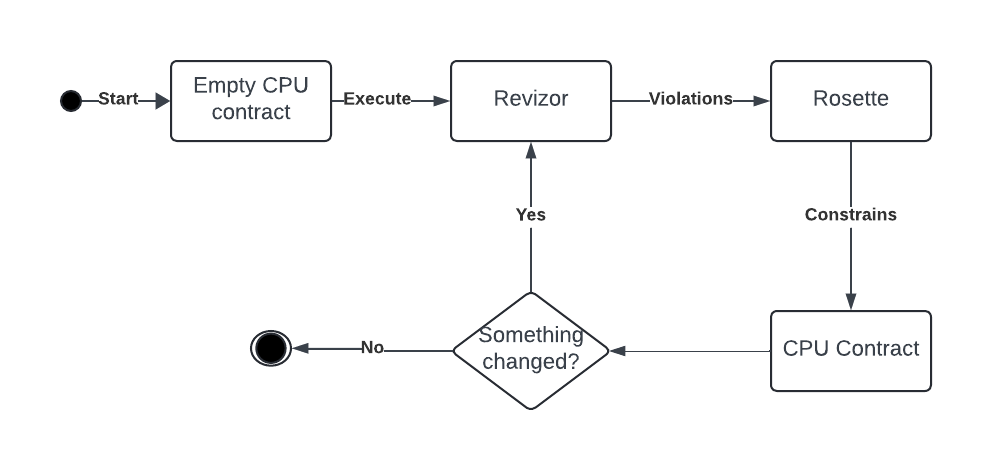
\includegraphics[width=.6\textwidth]{images/Thesis.png}
\end{center}

\section{DSL}
\label{cha:DSL} To represent the CPU contract, the researchers needed a language
that was able to describe the ISA of a CPU and its contract. To archieve this need,
at the beginning of the project, they developed aDomain Specific Language (DSL).
This language is able to define, check and evaluate a number of boolean conditions,
such as AND, OR, NOT, EQUAL, and to access CPU's registers. Here is a basic example
of a DSL code, that if a condition (that is always true in this case) is met, then
it traces the Program Counter (PC) register:

\begin{verbatim}
  (IF (BOOL #t) (REG 7)) # Register 7 is the PC
\end{verbatim}

This snippet is the most basic example of a CPU contract, that is used across the
project for testing purposes only.

The language was pretty easy to read and write, and did the job for the
bootstrapping of the project, and the first steps of research. This was enough
as a proof of concept to see wheather the whole system was working, but now with
the further steps of the project, this is not enough anymore. To have a more research-validated,
robust, complete and universal language, the team decided to switch from this
DSL to using the BIR language (more in Section \ref{cha:BIR}), and the whys in the
last section of this chapter (\ref{cha:Language comparison}).

\section{BIR}
\label{cha:BIR} Binary Intermediate Representation (BIR, \cite{bir_pub}) is a
descriptive language developed by a group of researchers, that were trying to make
analysis of binary files, with the goal of validating them. To do so, they
needed a language that was platform independent, and that represented the ISA of
a CPU. The goal of the language is to be clear, meaning that it has only explicit
type changes, leaving no room for side effects and abstracted behaviours. BIR has
functionalities such as blocks, jump, assignent and so on. In our project, the part
of BIR that was used are the expressions. When we talk about expressions in BIR
we mean the following possible statements:
\begin{itemize}
  \item \textbf{Constant}: A constant value, in most cases a numeric value.

  \item \textbf{Unary operation}: Operation performed on a singular value, such
    as binary NOT, or change sign operation.

  \item \textbf{Binary expressions}: Operation performed on two values,
    combining them, such as SUM, MULT and so on. The operators need to be compatible
    with one another, meaning they need to have the same binary precision

  \item \textbf{Binary Predicates}: A function that returns a boolean value computing
    from two values. An example is the EQ predicate, checking equality of two given
    values.

  \item \textbf{Variable}: Usage of variables, such as the value inside a given
    register, abstracting from the value itself.

  \item \textbf{IfThenElse statement}: A conditional statement with a condition,
    and two branches that are evaluated and executed according to the condition
    itself.

  \item \textbf{Load}: Load a value from a given memory address.

  \item \textbf{Store}: Store a value in a given memory address.

  \item \textbf{OPERAND-VALUE}: Returns the value of the operand for a given operation
    code

  \item \textbf{OPERAND-TYPE}: Returns the type of the operand for a given operation
    code

  \item \textbf{OPERAND-ACCESS}: Returns the access mode of the operand for a given
    operation code

  \item \textbf{OPCODE}: Returns the opcode of the instruction that has just been
    executed

  \item \textbf{SLIDE}: Slide the bits of a given value, extracting a range of
    bits from it.
\end{itemize}

Followig there is a simple example of each one of the possible expressions that
has been used in the project, with a brief comment on the meaning of them.
\begin{verbatim}
- (BExp_Const (bv 1 Bit32)) # Constant value 1, in binary vector of 32 bits.
- (BExp_UnaryExp (BIExp_ChangeSign (BExp_Const (bv 42 Bit8)))) # Change sign of 42
- (BExp_BinExp BIExp_Plus (BExp_Const (bv 12 Bit8)) (BExp_Const (bv 30 Bit8))) # Sum
of 12 and 30
- (BExp_BinPred BIExp_Equal (BExp_Const (bv 12 Bit8)) 
(BExp_Const (bv 30 Bit8))) # Check if 12 is equal to 30
- (BExp_Den (BVar REG 1)) # Value inside register R1
- (BExp_IfThenElse (BExp_BinPred BIExp_Equal (BExp_Const (bv 12 Bit8)) 
(BExp_Const (bv 30 Bit8))) (BExp_Const (bv 42 Bit8)) (BExp_Const (bv 50 Bit8))) 
# If 12 is equal to 30, return 42, else return 50
- (BExp_Load BExp_Den (BVar REG 1) (BExp_Const (bv 0 Bit32)) BEnd_LittleEndian Bit64) 
# Load value from memory address 0 in R1, in little endian, 64 bits
- (BExp_Store BExp_Den (BVar  REG 1) (BExp_Const (bv 0 Bit32)) BEnd_LittleEndian 
(BExp_Const(bv 2 Bit32))) # Store value 2 in memory address 0 in R1, in little endian
- (OPERAND-VALUE 1) # Return the value of the operand for the operation code 1
- (OPERAND-TYPE 1) # Return the type of the operand for the operation code 1
- (OPERAND-ACCESS 1) # Return the access mode of the operand for the operation code 1
- (OPCODE) # Return the opcode of the instruction that has just been executed
- (SLIDE 63 8 (OPERAND-VALUE 1)) # Used to extract a desired range of bits from a given address
\end{verbatim}

This range of expressions can also be nested and chained, to make more complex
constructs and represent more engineered ISAs, and for our purpose contracts.

As you might see, the language itself if extremely explicit, and understanding what
an instruction is supposed to do is extremely straight forward. The language is
almost overwhelmingly clear and reduntant, so that there are no doubts on what the
described expression does or means.

\section{Language comparison}
\label{cha:Language comparison} Multiple reason concurred to the decision of switching
from the DSL to BIR. Some of them are technical, while some are more research-based.

Starting with the technical side, the DSL was not an appropriate language from
the beginning. It did not implement the majority of the operations that a modern
processor can perform, failing in representing completely a CPU contract. This could
have been a huge limitation, since all this project aims to completely sintesise
a contract, and not having all the pieces to do so, would have been a limitation,
given the fact that vendors are using increasingly complex contracts. As
mentioned in \ref{cha:DSL}, the DSL was a good option for the beginning and the proof
of concept phase of the project, but could have never been enough for the final
goal of the project.

On the ohter hand, there is BIR. It is a language that, following modern CPU architecture,
is complete, and very explicit in its syntax. As we pointed out in previous
sections, while the DSL has a pretty simple syntax, BIR is more complex, probably
a bit harder to write, but way simpler and more clear to read. And since almost no
code for this project is going to be written by hand, this is a advantage that
BIR has. Also, the fact that BIR is complete makes it a better option, also for future
development, or current usage of the toolchain for more complex CPUs.

The DSL was also developed almost on the flight, for this specific project,
while BIR was created with the goal in mind to represent specifically and in a
more general fashion all CPU's ISA. BIR is therefore research-based, and
engineered for the purpose that we are aiming in this project. Even if this had never
been the case, such a lack of research in the DSL could have ment some
limitations in the future, or the need to change some parts of the code, slowing
down further development.

BIR has also the feature that all his expressions are explicit and platform
independent. This means that once I write my IfThenElse, the only code that gets
executed is that one, with no hidden behaviours or side effects, while this was
not explicitly the case for the DSL.

One last techical reason that played a major role in the choice, is the fact that
BIR's syntax is pretty close to a lot of dialects used in other security-related
tools. One good example is the Valgrind IR (\cite{valgrind}), a framework used for
dynamic analysis and threading bugs. Such a cohesion with already existing state-of-the-art
tooling would make the barrier to entry lower for other interested researchers
or security experts in the usage of this tool.

The last reason was that the BIR language created by some researchers that are
part of the project, and this would have made the integration of the language in
the project easier, and further development easier. This was therefore also a need
of the team, and not only a set of technical reasons. Having all the parties aligned
on the same language, meant more stability and long term sotenibility of the
project.

This is why, in the end, the team decided to pursue the migration.